{}\documentclass[letterpaper,
compress,
xcolor=x11names,
%draft,
]{beamer}
% Package imports
\usepackage{mathtools} % imports `amsmath'
\DeclareMathOperator{\sech}{sech}
\usepackage{amssymb}
\usepackage{fixltx2e}
\usepackage{lmodern}
\usepackage{movie15}
%\usepackage{media9}
\usepackage{microtype}
\usepackage{animate}
\usepackage{subcaption}
\captionsetup{compatibility=false}

% I just did this
\usepackage[english]{babel}
\usepackage[utf8]{inputenc}
\usepackage{amsmath}
\usepackage{graphicx}
\usepackage[colorinlistoftodos]{todonotes}
\usepackage{tikz}
\usetikzlibrary{tikzmark}
\usepackage{array}
\usepackage{layout}
\usepackage{multicol}
\usepackage{multirow}
\usepackage{booktabs}
%I just did this

% `beamer' configuration
\usefonttheme{professionalfonts}
\useoutertheme[subsection=false,]{miniframes}
\setbeamercolor*{alerted text}{fg=red}
\setbeamercolor*{example text}{fg=black}
\definecolor{CSU_green}{RGB}{30, 70, 43}
\definecolor{CSU_gold}{RGB}{200, 195, 114}
\setbeamercolor*{lower separation line head}{bg=CSU_gold}
\setbeamercolor*{section in head/foot}{fg=white,bg=CSU_green}
\setbeamercolor*{subsection in head/foot}{bg=white}
\setbeamercolor*{upper separation line head}{bg=CSU_gold}
\setbeamercolor*{page number in head/foot}{fg=CSU_green}
\setbeamercolor*{normal text}{fg=black,bg=white}
\setbeamercolor*{palette tertiary}{fg=black,bg=black!10}
\setbeamercolor*{palette quaternary}{fg=black,bg=black!10}
\setbeamercolor*{structure}{fg=black}
\setbeamerfont{frametitle}{shape=\scshape}
\setbeamerfont{institute}{shape=\scshape}
\setbeamerfont{section in head/foot}{shape=\scshape}
\setbeamerfont{subsection in head/foot}{shape=\scshape}
\setbeamertemplate{bibliography item}{}
\setbeamertemplate{itemize items}[ball]
\setbeamertemplate{navigation symbols}{}
\setbeamertemplate{footline}[frame number]
\usetikzlibrary{calc,arrows}
\graphicspath{{graphics/}{graphics/movies/}{graphics/images/}}
\usepackage{remreset}                  % hack to display beamer navigation
\makeatletter                          % circles even if not declaring
\@removefromreset{subsection}{section} % subsections
\makeatother                           % see: http://tex.stackexchange.com/a/2078
\setcounter{subsection}{1}             % see: https://bitbucket.org/rivanvx/beamer/issue/218

% `biblatex' configuration
\usepackage[backend=biber,
style=authortitle-comp,
]{biblatex}
\addbibresource{presentation.bib}

% `enumitem' configuration
\usepackage{enumitem}
\setlist[itemize,1]{label=\usebeamertemplate{itemize item}}
\setlist[itemize,2]{label=\usebeamertemplate{itemize subitem}}
\setlist[itemize,3]{label=\usebeamertemplate{itemize subsubitem}}
\DeclareMathOperator{\sinc}{sinc}


% `graphicx' configuration
\usepackage{graphicx}
\begin{document}
	\title{Functions, Nested Loops, and Recursion}
	%\subtitle{MATH-151:  Mathematical Algorithms in Matlab}
	\author{MATH-151:  Mathematical Algorithms in Matlab}
	\date[202X]{September 11, 2023}
	\titlegraphic{
\includegraphics[height = 3cm]{CSU_Ram_Logo.jpg}}



%%%%%%%%%%%%%%%%%%%%%%%%%%%%%%%%%%%%%%%%%%%%%%%%%%%%%%

\begin{frame}
\titlepage
\end{frame}
%%%%%%%%%%%%%%%%%%%%%%%%%%%%%%%%%%%%%%%%%%%%%%%%%%%%%%%%%
\section{Functions}

\begin{frame}{Why Use Functions?}
	\footnotesize
	\begin{itemize}
		\item A lot of time when writing longer pieces of code, there will be repeated blocks of code. Functions allow us to make our code more readable by replacing these repeated blocks of code with a single line that tells Matlab to perform that block.
		\item<2-> For example, \texttt{sin(x)} informs Matlab to do a Taylor Series sum to approximate the $sin(x)$ function.
		\begin{itemize}
			\item It is much more less cluttered to see just \texttt{sin(x)}, rather than a loop, many times.
			\item Furthermore, we would see \texttt{factorial(n)} in each loop of that sum, which is another function that replaces a set of code! 
		\end{itemize}
		\item<3-> Matlab has many built-in functions to perform commonly seen computations, but it also allows us to create our own functions! 
	\end{itemize}
\end{frame}

%%%%%%%%%%%%%%%%%%%%%%%%%%%%%%%%%%%%%%%%%%%%%%%%%%%%%%%%%

\begin{frame}{Structure of a Function}
	\footnotesize
	\begin{itemize}
		\item Similar to a script a function is a .m file in Matlab however we need to inform Matlab that is is a function. So each function code needs to begin with a line like below\\
		\texttt{\textcolor{blue}{function} output = function\_name(input)}
		\begin{itemize}
			\item<2-> \textcolor{blue}{function} tells Matlab that we are beginning to define a function
			\item<3-> \texttt{output} tells Matlab what the result of the function is, everything else will be deleted from memory when the function is completed
			\item<4-> \texttt{function\_name} is the name used for the function call in another piece of code telling Matlab when to run this block of code. The filename for this function should match the function name, so this file would be named function\_name.m
			\item<5-> \texttt{input} is the input to the function, the code should be expected to run with only the given inputs.
		\end{itemize}
		\item<6-> It is usually good commenting practice to include a preamble describing the function's use and format of the input and output variables.
	\end{itemize}
\end{frame}

%%%%%%%%%%%%%%%%%%%%%%%%%%%%%%%%%%%%%%%%%%%%%%%%%%%%%%%%%
\begin{frame}{Function Example}
	Here is an example script for a function to calculate your grade in this class
	\begin{center}
		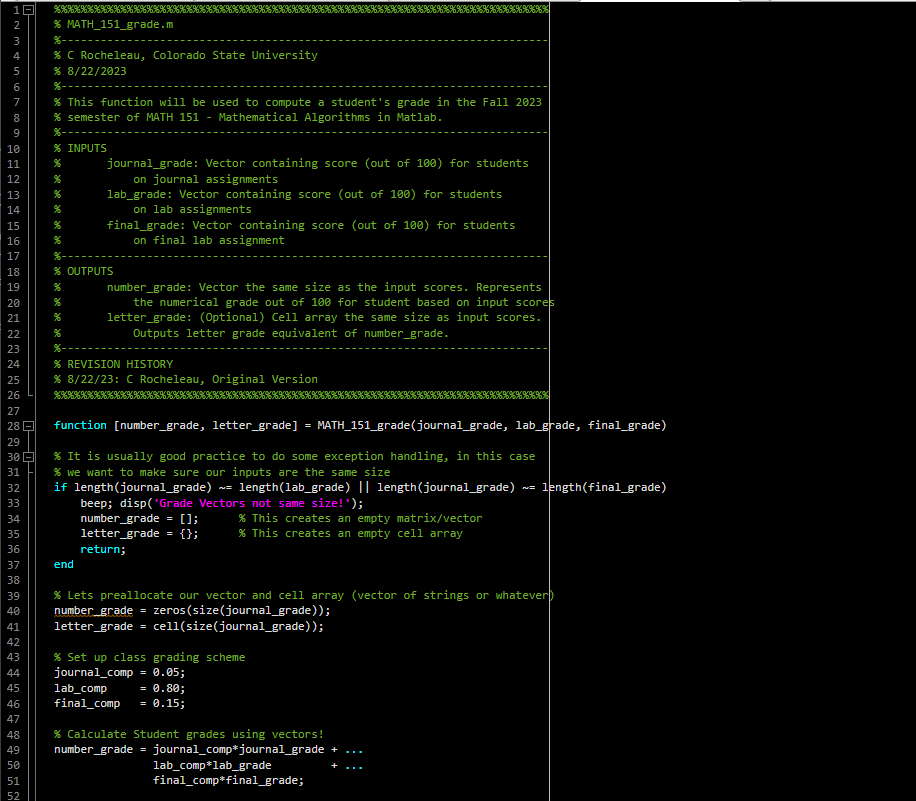
\includegraphics[height = 5.5cm]{function_example.png}
	\end{center}
	Wait a second, what's going on with the inputs and outputs? Can you have more than one of each?
\end{frame}

%%%%%%%%%%%%%%%%%%%%%%%%%%%%%%%%%%%%%%%%%%%%%%%%%%%%%%%%%

\begin{frame}{Multiple Inputs or Outputs}
	\footnotesize
	\begin{itemize}
		\item If needed, we can allow a function to have multiple outputs, as well as accept multiple inputs.
		\begin{itemize}
			\item Be careful, the ordering is important!
		\end{itemize}
		\item<2-> To have multiple outputs, we place them in square brackets, [...], where each output variable is separated with a comma \\
		\hspace{0.5cm}\texttt{[number\_grade, letter\_grade]}
		\item<3-> Similarly, to have multiple inputs we list them in the parentheses of the function call. Again, separated by commas\\
		\hspace{0.5cm}\texttt{(journal\_grade, lab\_grade, final\_grade)}
		\begin{center}
			\includegraphics[width = \linewidth]{multiple_IO.png}
		\end{center}
		\item<4-> Inputs may be treated as optional in the function, or outputs may be optional when calling the function, for example \\
		\hspace{0.5cm}\texttt{number\_grade = MATH\_151\_grade(100,100,100)} \\
		will only output the number grade
		
	\end{itemize}
\end{frame}

%%%%%%%%%%%%%%%%%%%%%%%%%%%%%%%%%%%%%%%%%%%%%%%%%%%%%%%%%

\begin{frame}{Subfunctions}
	\footnotesize
	\begin{itemize}
		\item Sometimes we will have a repeated block of code inside a function
		\begin{itemize}
			\item That sounds like a job for a function!
		\end{itemize}
		\item<2-> When needed, we can put multiple functions in the same file, if the primary function needs additional function calls.
		\begin{itemize}
			\item For example, my simulation's physics model function had a subfunction for computing the amount of force each thruster created, rather than copy the same block of code for each of the 4 thrusters!
		\end{itemize}
		\item<3-> Creating a subfunction is just like creating a function, the only difference is that we need to make sure that the functions are given \textcolor{blue}{\texttt{end}} statements, so Matlab knows when one function ends and the other begins.
	\end{itemize}

	\onslide<4->{We'll see an example of this shortly, but while we're talking about functions inside functions...}
\end{frame}

%%%%%%%%%%%%%%%%%%%%%%%%%%%%%%%%%%%%%%%%%%%%%%%%%%%%%%%%%
\section{Nested Loops}

\begin{frame}{Loops in Loops}
	\footnotesize
	\begin{itemize}
		\item In many real-world cases, we deal with multivariable functions. In those cases, we don't just have a single \texttt{x} that we need to iterate across, we also have a \texttt{y} that varies as well. 
		\item To calculate all combinations of values from \texttt{x} and \texttt{y} we need to use a \textbf{nested loop}
		\begin{itemize}
			\item This means that we have a loop inside of a loop
			\item We hold the \texttt{x} value constant and iterate across all the \texttt{y} values, then we move onto the next \texttt{x} value and repeat.
		\end{itemize}
		\item<2-> Suppose we have a grid of points and want to find the angle to each of them from the origin.
	\end{itemize}
	\begin{center}
		\onslide<2->{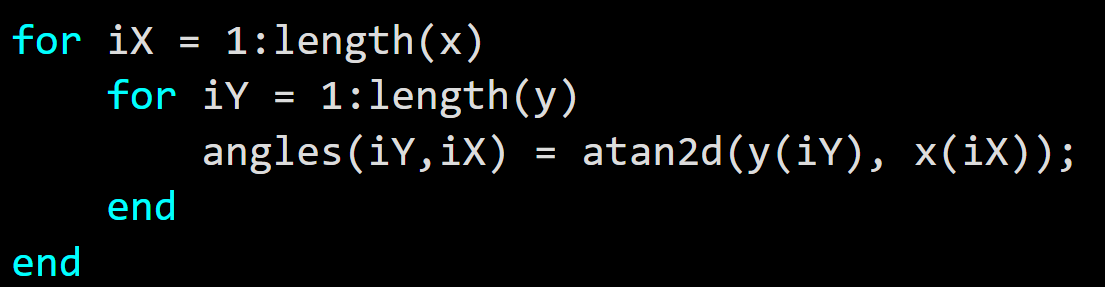
\includegraphics[height = 2cm]{angle_nested_loop.png}
		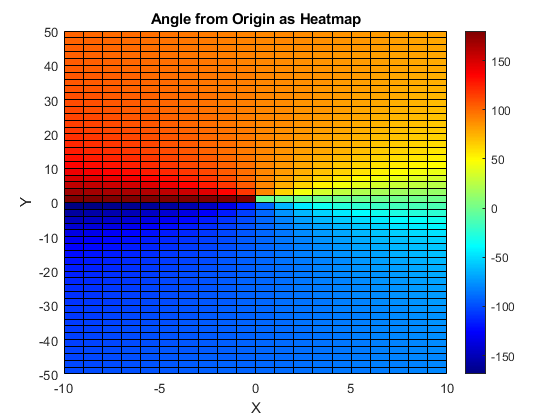
\includegraphics[height = 2cm]{angle_surface.png}}
	\end{center}
\end{frame}

%%%%%%%%%%%%%%%%%%%%%%%%%%%%%%%%%%%%%%%%%%%%%%%%%%%%%%%%%

\begin{frame}{Data Matrices}
	\footnotesize
	\begin{itemize}
		\item This can also be used for Data Matrices. Each row is a different variable, and each column is a different subject.
		\item We can use a nested loop to perform our Gambler's Ruin game many times and collect statistics!
		\begin{center}
			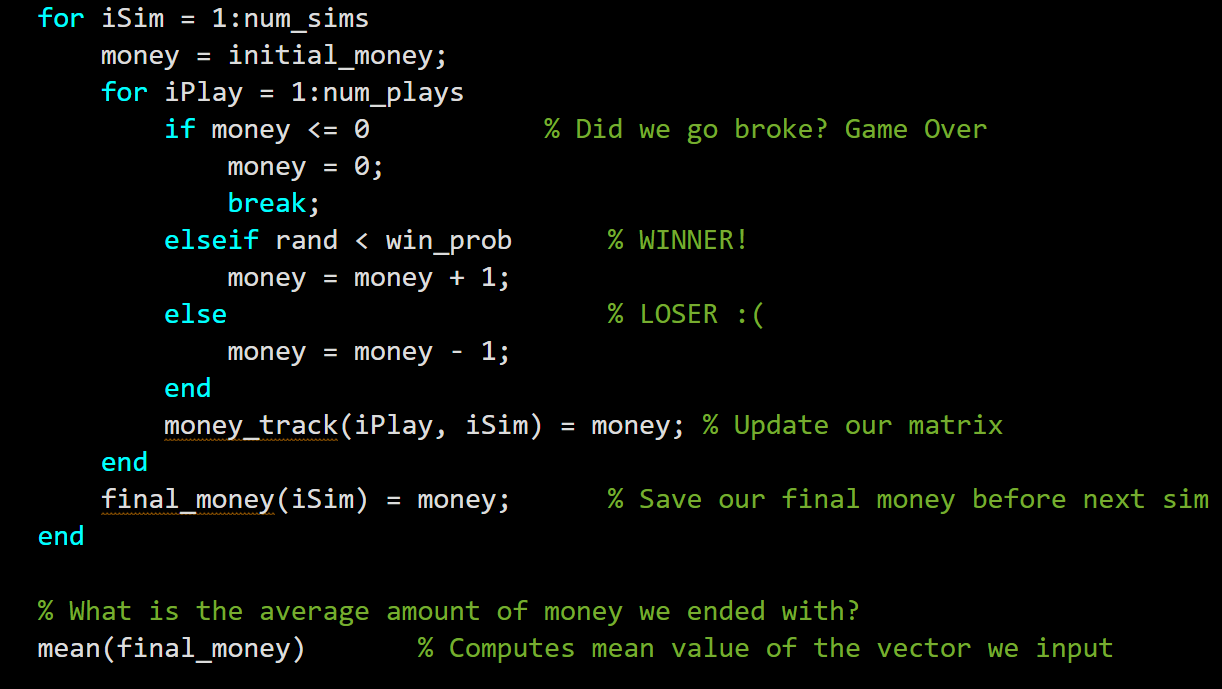
\includegraphics[width = 7cm]{gamblers_ruin.png}
		\end{center}
		\item In this game we had an average final money count of \$5.31
	\end{itemize}
\end{frame}

%%%%%%%%%%%%%%%%%%%%%%%%%%%%%%%%%%%%%%%%%%%%%%%%%%%%%%%%%
\section{Recursion}

\begin{frame}{Recursive Relationships}
	\footnotesize
	\begin{itemize}
		\item In some algorithms we will run into each step will be a tiny version of the algorithm itself. For example, when doing $n!$ we will need to find $(n-1)!$, which means we'll need to find $(n-2)!$, and so on. 
		\item<2-> In these cases, rather than writing a loop, we can create a \textbf{recursive function}
		\begin{itemize}
			\item This is a function that calls on itself
			\item<3-> Each time we call the function, we will get closer to some base case
			\item<3-> The answer will ``flow up" through all the previous function calls to give us our desired result in the end.
		\end{itemize} 
	\end{itemize}
	\begin{center}
		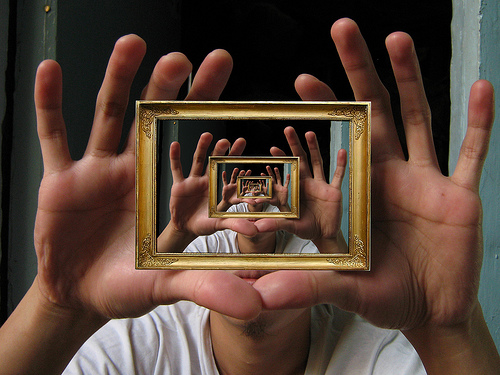
\includegraphics[width = 5cm]{recursion_mirror.jpg}
	\end{center}
\end{frame}

%%%%%%%%%%%%%%%%%%%%%%%%%%%%%%%%%%%%%%%%%%%%%%%%%%%%%%%%%

\begin{frame}{Bisection Method}
	\footnotesize
	\begin{itemize}
		\item This is an algorithm for finding the root, $f(x) = 0$ of an equation
		\item Suppose we know $f(a)$ is negative and $f(b)$ is positive. If $f$ is a continuous function, is must pass through 0 between $a$ and $b$.
		\item<2-> So we cut it in half and try $f(m)$, where $m  =\frac{a+b}{2}$
		\begin{itemize}
			\item<3-> If it has the same sign as $f(a)$, $m$ becomes our new $a$
			\item<3-> If it has the same sign as $f(b)$, $m$ becomes our new $b$
		\end{itemize} 
		\item<4-> This gives us a new, smaller possible range, so we do Bisection Method on that range
		\item<4-> We continue until $f(m)$ is sufficiently small.
	\end{itemize}
	\begin{center}
		\onslide<4->{
		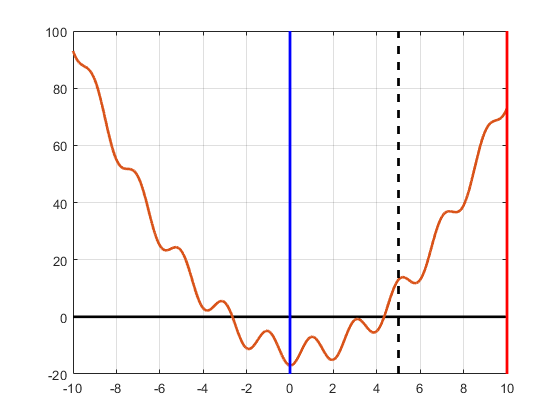
\includegraphics[height = 1.75cm]{bisection_img1.png}
		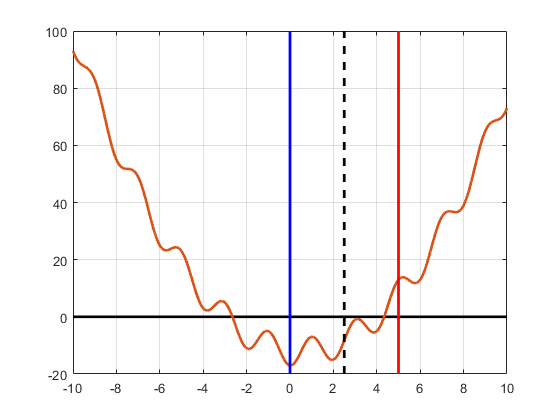
\includegraphics[height = 1.75cm]{bisection_img2.png}
		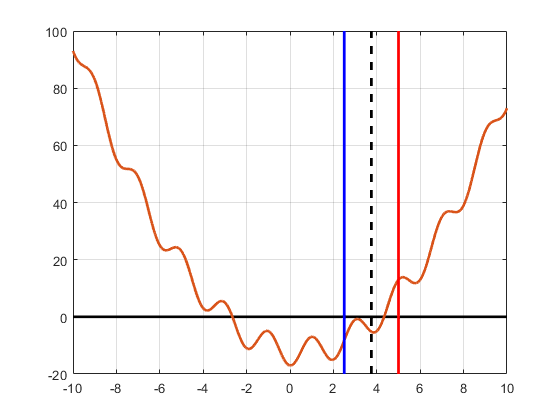
\includegraphics[height = 1.75cm]{bisection_img3.png}
		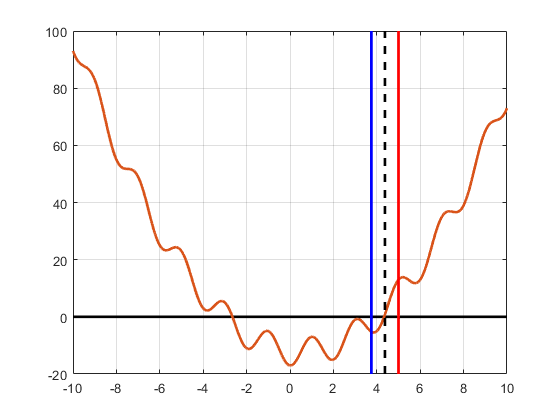
\includegraphics[height = 1.75cm]{bisection_img4.png}}
	\end{center}
\end{frame}

%%%%%%%%%%%%%%%%%%%%%%%%%%%%%%%%%%%%%%%%%%%%%%%%%%%%%%%%%
\end{document}